\chap{Un robot de compagnie}\label{ch.pet}

Un \textit{robot autonome} adopte un comportement spécifique en fonction de la situation dans laquelle il se trouve. Il réussi à réagir grâce au \textit{feedback}, littéralement de l'information en retour. Il faut donc que le robot puisse "voir" le monde qui l'entoure pour pouvoir y régir.

\sect{Thymio vous obéi}

Pour commencer, nous allons dresser Thymio pour qu'il vous obéisse. 

\begin{bclogo}[couleur = pink!30, arrondi = 0.1, logo = \bccrayon, ombre = true]{Challenge!}Écrivez un programme en utilisant VPL qui fait avancer Thymio lorsque vous mettez votre main devant lui!
\end{bclogo}

Il y a cinq capteurs de distance devant Thymio et deux derrière. Ce sont les même que ceux qui se trouve sous Thymio et que nous avons utilisé pour détecter une table! Avancez votre main en direction des capteurs devant Thymio, vous verrez une lumière rouge apparaître à côté du capteur qui vous aura détecté, comme sur \cref{fig.detect}.

\begin{figure}
\begin{center}
\gr{detect}{.6}
\caption{L'avant de Thymio. Deux doigts sont détectés par les capteurs avant.}\label{fig.detect}
\end{center}
\end{figure}

Le bloc \blk{event-prox} sert à utiliser les capteurs avants et arrières de Thymio. Les cases sont utilisées comme avec les détecteurs en dessous de Thymio. En cliquant dessus, ils passent de gris à blanc, à rouge et à nouveau à gris. Nous redonner les significations des couleurs en dessous:

\begin{description}
	\item[Gris] \hfill \\
		Le détecteur n'est pas utilisé
	\item[Rouge] \hfill \\
		L'événement associé est déclenché si un objet se trouve proche de Thymio
	\item[Blanc] \hfill \\
		L'événement associé est déclenché si aucun objet ne se trouve proche de Thymio
\end{description}

Pour faire avancer Thymio si votre main est proche de lui et le faire s'arrêter si elle est loin, il nous faudra deux paires événement-action, comme sur \cref{fig.follow-hand}. La première dit à Thymio de s'arrêter s'il ne détecte rien devant lui grâce au bloc capteur dont le carré central est blanc et au bloc moteur dont les \textit{sliders} sont au centre des barres. La deuxième paire dit qu'il doit avancer s'il voit quelque chose devant lui grâce au bloc capteur dont le carré central est rouge et au bloc moteur avec les \textit{sliders glissés vers le haut}.

\begin{figure}[h]
\begin{center}
\gr{likes-forward}{.4}
\caption{Thymio avance vers votre main}\label{fig.follow-hand}
\end{center}
\end{figure}

\sect{Faire tourner Thymio}

Thymio n'est pas comme une voiture, il n'a pas de volant, ni de roues directrices. Pour tourner, il doit simplement faire tourner ses deux roues à des vitesses différentes! On appelle cela la \textbf{direction différentielle}, ou \textbf{differential drive}. Cette façon de se diriger est utilisée par de nombreux véhicules, comme par exemple le bulldozer de \cref{fig.bull}.

\begin{figure}
\begin{center}
\gr{bulldozer}{0.25}
\caption{Un bulldozer qui utilise aussi  la \textbf{direction différentielle}}\label{fig.bull}
\end{center}
\end{figure}

Si la roue droite tourne plus vite que la roue gauche, alors Thymio tournera à gauche, tandis que si sa roue gauche tourne plus vite que sa roue droite, il tournera à droite. Plus la différence de vitesse est élevée, plus le virage sera serré. Et pour tourner sur lui-même, il lui suffit de faire tourner ses deux roues à la même vitesse mais dans des sens opposés!

En réglant le bloc vitesse avec les \textit{sliders} à des endroits différents, les roues de Thymio ne tourneront pas à la même vitesse, ce qui le fera tourner. Essayez de régler le bloc vitesse comme cela: \blk{turning}. Si vous chargez ensuite ce programme et appuyez sur le bouton central, Thymio devrait tourner sur lui-même. Vous pouvez toujours l'arrêter en appuyant sur \blksm{stop}.

\begin{bclogo}[couleur = blue!30, arrondi = 0.1, logo = \bcinfo, ombre = true]{Truc et astuce!}Le bloc vitesse s'anime dès que vous régler les \textit{sliders} pour vous donner une idée du mouvement de Thymio!
\end{bclogo}

\sect{Thymio vous suit}

Un vrai animal de compagnie ne se contente pas de s'approcher ou de s'éloigner de vous, il vous suit un peu partout! 

\begin{bclogo}[couleur = pink!30, arrondi = 0.1, logo = \bccrayon, ombre = true]{Challenge!}Écrivez un programme en utilisant VPL qui fait avancer Thymio lorsque vous mettez votre main devant lui et qui le fait tourner si vous tournez autour de lui!
\end{bclogo}

{\raggedleft \hfill Programme \bu{likes.aesl}}

Pour que Thymio puisse vous suivre plus fidèlement, il faudra encore ajouter deux paires événement-action au programme précédant. S'il vous détecte avec son capteur avant-droit, il doit tourner à droite et s'il vous détecte avec son capteur avant-gauche, il doit tourner à gauche.

Vous pouvez essayer différentes vitesses, le faire tourner sur lui-même ou non, afin de trouver le meilleur compromis! 

Une façon de faire est illustrée sur \cref{fig.likes}.

\begin{figure}
\begin{center}
\gr{likes-turns}{0.4}
\caption{Thymio s'oriente face à vous}\label{fig.likes}
\end{center}
\end{figure}

\sect{Thymio vous fui}

Parfois, même le plus fidèle animal de compagnie n'a pas envie de vous suivre. 

\begin{bclogo}[couleur = pink!30, arrondi = 0.1, logo = \bccrayon, ombre = true]{Challenge!}Écrivez un programme en utilisant VPL qui fait reculer Thymio lorsque vous mettez votre main devant lui et qui le fait vous éviter si vous lui tournez autour!
\end{bclogo}

{\raggedleft \hfill Programme \bu{does-not-like.aesl}}

Pour réussir à donner ce  comportement à Thymio, il suffit simplement de régler les moteurs sur la marche arrière s'il vous détecte avec son capteur avant et d'échanger les événements des paires d'événement-action restantes du programme précédant, comme sur \cref{fig.recule-evite}.

\begin{figure}[h]
    \centering
    \subfigure[S'il vous détecte devant lui, il recule]{ \label{fig.recule} 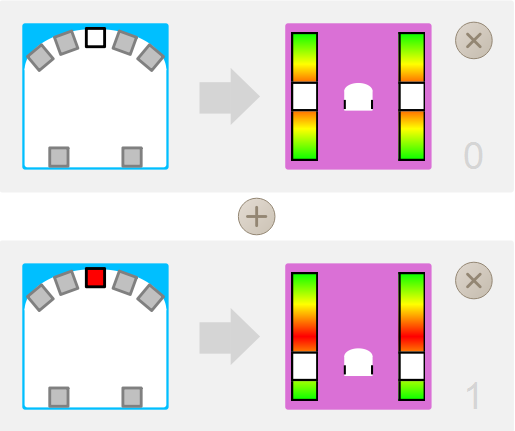
\includegraphics[width = 0.35\textwidth]{Thymio-fui}}
    \hspace{1cm}
    \subfigure[S'il vous détecte sur les côtés, il vous évite]{ \label{fig.evite} 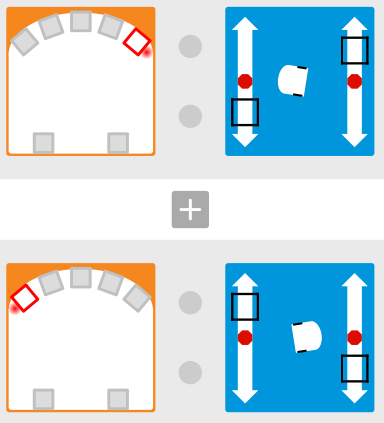
\includegraphics[width = 0.35\textwidth]{hates}}
    \caption{Thymio vous évite et vous fui}
    \label{fig.recule-evite}
\end{figure}

\begin{bclogo}[couleur = pink!30, arrondi = 0.1, logo = \bccrayon, ombre = true]{Challenge!}Jouez avec les différents capteurs avant de Thymio. Vous pouvez utiliser les capteurs jusque là inutilisés pour améliorer le comportement de Thymio!
\end{bclogo}

\sect{Régler les \textit{sliders} plus précisément (avancé)}

Ce n'est pas très facile de régler les \textit{sliders} précisément pour, par exemple, faire avancer Thymio tout droit. Si vous regardez dans la fenêtre principale d'Aseba, vous verrez que le code qui sera transmis à Thymio s'écrit tout seul dès que vous remplissez les paires événement-action dans VPL. En comprenant un peu ce code et en le modifiant directement, il est possible d'ajuster plus précisément les vitesse des roues!

Le \cref{Follower_code} avec la figure d'à côté vous montre un exemple!

\begin{wrapfigure}{r}{0.24\textwidth}
  \begin{center}
    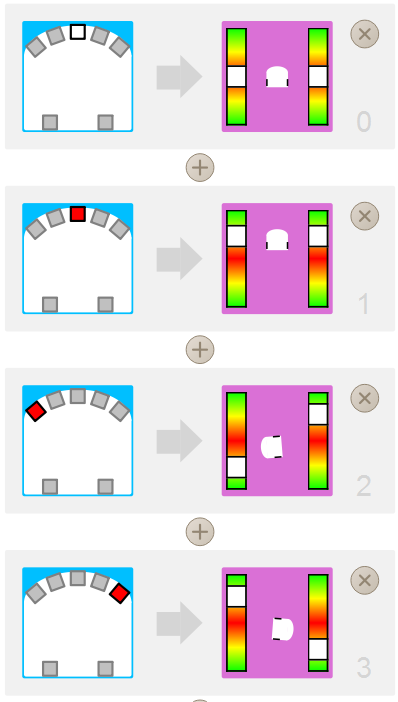
\includegraphics[width=0.24\textwidth]{follow4}
  \end{center}
\end{wrapfigure}

\begin{small}
\begin{lstlisting}[frame=single, caption={Thymio vous suit}, label=Follower_code, linewidth=9cm] 

onevent prox
	if prox.horizontal[2] < 400 then
		motor.left.target = 0
		motor.right.target = 0
	end
	if prox.horizontal[2] > 500 then
		motor.left.target = 300
		motor.right.target = 300
	end
	if prox.horizontal[0] > 500 then
		motor.left.target = -350
		motor.right.target = 350
	end
	if prox.horizontal[4] > 500 then
		motor.left.target = 350
		motor.right.target = -350
	end

\end{lstlisting}
	\end{small}

La ligne \p{onevent prox} signifie que le code qui suit sera lancé lorsque l'événement lié aux capteurs de proximité se produira. Cet événement est simplement une lecture de tous les capteurs qui a lieu dix fois par seconde!

Ensuite, lorsque l'événement se produit, Thymio teste la valeur des capteur avec la condition: \p{if \ldots  then \ldots  end}. Il commence par tester le capteur numéro 2 comme nous le voyons avec la phrase \p{prox.horizontal[2]}. Si cette valeur est inférieure à 400, alors (\p{then}), Thymio règle la vitesse des moteurs gauche et droite à 0 avec les phrases: \p{motor.left.target = 0} et \p{motor.right.target = 0}.

Chaque bloc \p{if \ldots  then \ldots  end} teste un capteur spécifique et effectue ou non l'action associée. C'est exactement comme sur la figure à droite du \cref{Follower_code}.

\begin{enumerate}
	\item Thymio teste si rien ne se trouve devant lui, si c'est le cas, il s'arrête
	\item Thymio teste si quelque chose se trouve devant lui, si c'est le cas, il avance
	\item Thymio teste si quelque chose se trouve à sa gauche, si c'est le cas, il tourne à gauche
	\item Thymio teste si quelque chose se trouve à sa droite, si c'est le cas, il tourne à droite
\end{enumerate}

Nous voyons donc que chaque paire événement-action correspond à un bloc \p{if \ldots  then \ldots  end}!

Finalement, une fois que Thymio a testé tous ces capteurs, il attend le prochain événement \p{prox} et recommence ses tests, etc\ldots

Si vous voulez, vous pouvez essayer de modifier les nombres après les symboles $<$ ou $>$, ou encore ceux après les signes $=$. Chacun d'eux ont leur utilité et leurs limites, essayez de les comprendre!

Vous ne pourrez pas modifier le code écrit si VPL est ouvert. Sauvegardez votre travail sur VPL et quitter cette fenêtre pour commencer à jouer avec la programmation écrite!